\documentclass{article}

\usepackage[utf8]{inputenc} 
\usepackage[russian]{babel}

\usepackage{listings}
\usepackage{float}
\usepackage{amsmath}
\usepackage{breqn}
% allow utf-8 input
\usepackage{url}            % simple URL typesetting
\usepackage{booktabs}       % professional-quality tables
\usepackage{amsfonts}       % blackboard math symbols
\usepackage{subcaption}
\usepackage[labelformat=parens,labelsep=quad,skip=3pt]{caption}
\usepackage{graphicx}
\usepackage{color}

\usepackage{mathtools}

\usepackage{geometry} % Меняем поля страницы
\geometry{left=2cm}% левое поле
\geometry{right=2cm}% правое поле
\geometry{top=3cm}% верхнее поле
\geometry{bottom=2cm}% нижнее поле

\newtheorem{theorem}{Теорема}
\newtheorem{definition}{Опредление}
\newcommand\scalemath[2]{\scalebox{#1}{\mbox{\ensuremath{\displaystyle #2}}}}

\addto\captionsrussian{\def\refname{Список используемой литературы}}

\newcounter{totreferences}

\pretocmd{\bibitem}{\addtocounter{totreferences}{1}}{}{}


\definecolor{deepblue}{rgb}{0,0,0.5}
\definecolor{deepred}{rgb}{0.6,0,0}
\definecolor{deepgreen}{rgb}{0,0.5,0}

\DeclareFixedFont{\ttb}{T1}{txtt}{bx}{n}{12} % for bold
\DeclareFixedFont{\ttm}{T1}{txtt}{m}{n}{12} 

\lstset{
language=Python,
basicstyle=\ttm,
otherkeywords={self},             % Add keywords here
keywordstyle=\ttb\color{deepblue},
emph={MyClass,__init__},          % Custom highlighting
emphstyle=\ttb\color{deepred},    % Custom highlighting style
stringstyle=\color{deepgreen},
frame=tb,                         % Any extra options here
showstringspaces=false            % 
}

\title{Заголовок}

\begin{document}

\tableofcontents

\newpage

\section{Введение}
Целью данного проекта является расчет некоторых параметров открытого планарного диэлектрического волновода. Проект командный, и подразумевает собой равный вклад всех 4х участников. Изначально, в ходе
работы над проектом я планирую взять на себя следующие задачи:
\begin{itemize}

 \item  Написание отчетов(презентации для проектной группы 1, промежуточные отчеты с результатами расчетов, финальный отчет-курсовая)
 \item  Разработка кода для нахождения общего решения дифф. уравнений в среде SymPy и Wolfram Mathematica.
 \item  Ручная валидация общих решений дифф. уравнений, полученных в системах символьных вычислений.
   
\end{itemize}
Ожидается, что в ходе командной работы над проектом мы научимся координировать свои усилия, а
именно формировать план работ, формировать задачи исходя из плана и распределять задачи между собой.
От данного курса я ожидаю получить навыки работы в команде и умение управлять своим временем. Под
этим я понимаю умение делигировать задачи со-командникам, представлять и обьяснять результаты своей
работы а так же умение разбираться в чужом коде и математических выкладках. Эти умения крайне полезны,
поскольку в современном мире технические проекты становятся все сложнее и сложнее. Потому, выполнение
современных исследованиний и разработок в одиночку практически крайне затруднительно. Особенно при
условии сжатых сроков и дефицита таких ресурсов как информация/тех. обеспечение. Данный проект как
раз и позволяет создать похожую ситуацию: сжатые временные рамки, сложность поставленной задачи.\\[10pt]
Относительно технических навыков я ожидаю улучшить свой навык работы с системами символьных
вычислений. Современные задачи моделирования, такие как моделирование распределения тепла на обшивке космических аппаратов, расчет температурных деформаций, моделирование процессов с радиоактивными материалами требуют больших вычислительных мощностей. Для создания таких моедлей используется
параллельное программирование, аппаратное ускорение и так же - символьные вычисления. Современные
математические пакеты, такие как Matlab Wolfram Mathematica представляют собой комплексные системы,
включающие полноценный язык программирования и набор вспомогателньых библиотек для компьютерной
алгебры, символьных вычислений, статистики, симуляций, анализа данных. В нашем проекте мы используем
Wolfram Mathematica и библиотеку символьных вычислений SymPy для языка Python.
\newpage

\section{Теоретическая часть}

Линза Люнеберга — линза, в которой показатель преломления не является постоянным, а изменяется по некоторому закону в зависимости от расстояния от центра в сферических или от оси в цилиндрических линзах. Обычно закон изменения показателя преломления подбирается таким образом, чтобы при прохождении линзы параллельные лучи фокусировались в одной точке на поверхности линзы, а испущенные точечным источником на поверхности — формировали параллельный пучок.

Подобная конструкция линз была впервые предложена немецким/американским математиком Рудольфом Люнебергом.\\[10pt]

\begin{figure}[H]
    \centering
    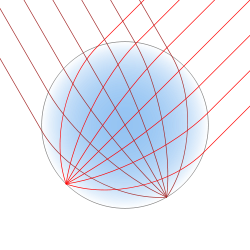
\includegraphics[width=120]{image3.png}
    \caption{}
    \label{tok_per_tweet}
\end{figure}

Линзы Люнеберга широко используются в СВЧ-технике. Одним из таких использований является создание сильно отражающих радиоволны объектов. В частности, линзы Люнеберга используются в ракетах-мишенях для имитации эффективной площади рассеяния реальных целей с бо́льшими размерами (например, боевых самолётов].

Использованию подобных линз в оптической технике препятствуют технические сложности изготовления линз с переменным показателем преломления, что определяет их высокую стоимость. Иногда для упрощения технологии производства подобные линзы собирают из дискретных элементов — небольших кубиков с различными показателями преломления.\\[10pt]

Линза Люнеберга долгое время оставалась не более чем математическим курьёзом, пока в начале 1960-х годов не была использована в качестве формирователя луча в американском радаре AN/SPG-59.

Радар AN/SPG-59 был одним из первых в мире радаров с фазированной антенной решёткой (ФАР). В отличие от современных радаров с ФАР, где пространственная картина луча формируется с помощью управляемых фазовращателей, в радаре AN/SPG-59 использовалась линза Люнеберга, расположенная в надстройке корабля. Выбор этой технологии был обусловлен отсутствием в 1960-х годах компактных и надёжных фазовращателей C-диапазона.

На поверхности линзы располагалось несколько тысяч приёмных и передающих элементов. Когда один из передающих элементов формировал на поверхности линзы сферическую радиоволну, линза преобразовывала её в волну с плоскопараллельными фронтами, фазовая картина которой снималась приёмными элементами и транслировалась на сферический излучатель, расположенный на вершине колоколообразной надстройки. Таким образом, сферический излучатель формировал в пространстве луч, направление которого соответствовало положению на линзе излучающего элемента.

\newpage

\section{Постановка задач}
В ТОВЛ Люнеберга распространение излучения можно описать уравнениями Максвелла.

\begin{figure}[H]
    \centering
    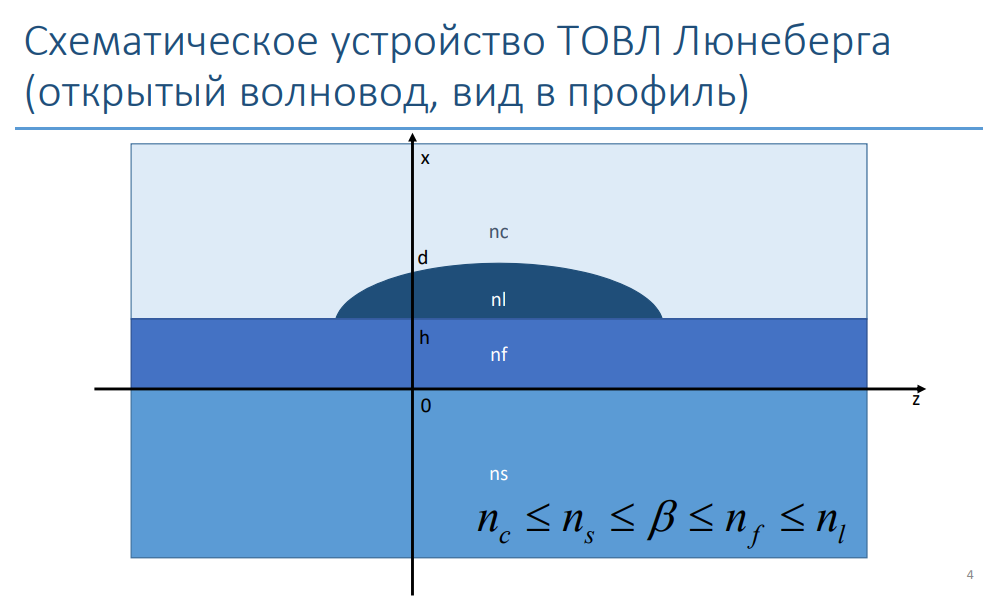
\includegraphics[width=\linewidth]{image2.png}
    \caption{Схематический вид ТОВЛ Люнеберга}
    \label{luneberg}
\end{figure}

\begin{definition}
{\bf Уравнения Максвелла} — система уравнений в дифференциальной или интегральной форме, описывающих электромагнитное поле и его связь с электрическими зарядами и токами в вакууме и сплошных средах.
\end{definition}

В нашей работе мы будем рассматривать трехслойник, который отличается от ТОВЛ Люнеберга, представленной на Рис. (2), отсутствием слоя $l$. На рисунке: $n_\tau, \tau = s, f, c$ - оптический показатель преломления в каждом соотв. слое.


\subsection{Формулировка Уравнений Максвелла}
В отсутствии внешних токов данные уравнения записываются в следющей форме\cite{luneberg2010}:
$$rot \vec{E} = - \frac{\mu}{c} \cdot \frac{\partial \vec{H}}{\partial t}$$
$$rot \vec{H} = \frac{\varepsilon}{c}\cdot\frac{\partial \vec{E}}{\partial t}$$

Где $\vec{E}$ - напряженность электрического поля, а $\vec{H}$ - напряженность магнитного поля. $c$ - скорость света в вакууме, $\mu$ - магнитная проницаемость, $\varepsilon$ - диэлектрическая проницаемость.

\par Общие решения уравнений максвелла являются полями мод плавно-нерегулярного волновода в адиабатическом приближении. Они имеют следующий вид:

$$\vec{E}(x, y, z, t) = \vec{E}(x, y, z) \cdot \frac{exp(i \omega t - i \phi(y, z))}{\sqrt{\beta(y, z)}}$$

$$\vec{H}(x, y, z, t) = \vec{H}(x, y, z) \cdot \frac{exp(i \omega t - i \phi(y, z))}{\sqrt{\beta(y, z)}}$$

где, $\beta(y, z) = \frac{1}{k_0} \sqrt{(\frac{\partial \phi}{\partial y})^2 + (\frac{\partial \phi}{\partial z})^2}$ - коэффициент фазового замедления, $k_0 = \frac{2\pi}{\lambda} = \frac{\omega}{c}$ - модуль волнового вектора. $\lambda$ - длина волны света.

Для данных полей справедливы следующие граничные условия:
\begin{itemize}
    \item Общие для TE,TM-мод:
    $$\vec{E}_\tau |_{x - 0} = \vec{E}_\tau |_{x + 0}, \vec{H}_\tau |_{x - o} = \vec{H}_\tau|_{x + 0} \eqno(1.a)$$
    \item Для TE-мод:
    $$\vec{H}_z|_{h-0} = \vec{H}_z|_{h+0}, \vec{E}_y|_{h-0} = \vec{E}_y|_{h + 0} \eqno(1.b)$$
    \item Для TM-мод:
    $$\vec{E}_z|_{h-0} = \vec{E}_z|_{h+0}, \vec{H}_y|_{h-0} = \vec{H}_y|_{h + 0} \eqno(1.c)$$
    \item Условие на бесконечности:
    $$|\vec{E}_\tau|_{x \to \pm \infty} < +\infty, |\vec{H}_\tau|_{x \to \pm\infty} < + \infty \eqno(1.d)$$
\end{itemize}

\subsection{СЛАУ для амплитудных коэффициентов}
В нулевом приближении асимптотического метода волновые уравнения для мод в каждом слое принимают следующий вид\cite{sevas2013}:

$$\frac{d^{2}E_{z}}{dx^{2}}+k_{0}^{2}\left(\varepsilon _{j}\mu_{j}-\beta ^{2}  \right)E_{z}=0 \eqno(1.1)$$

$$\frac{d^{2}H_{z}}{dx^{2}}+k_{0}^{2}\left(\varepsilon _{j}\mu _{j}-\beta ^{2} \right)H_{z}=0\eqno(1.2)$$

$$E_{y}=\frac{1}{k_{0}^{2}\left(\varepsilon \mu -\beta_{z}^{2} \right)}\left(\iota k_{0}\mu \frac{dH_{z}}{dx}\right)\eqno(1.3)$$

$$H_{y}=\frac{1}{k_{0}^{2}\left(\varepsilon \mu -\beta_{z}^{2} \right)}\left(-\iota k_{0}\varepsilon \frac{dE_{z}}{dx}  \right)\eqno(1.4)$$

{\bf Введем обозначения:}

$$
\gamma_\tau = k_0 \cdot \sqrt{\beta^2 - n_\tau^2}, \tau = s, f, c
$$
$$
\chi_\tau = k_0 \cdot \sqrt{n_\tau^2 - \beta^2}, \tau = s, f, c
$$

ФСР уравнения (1) (для $E_z$) каждом слое имеет вид \cite{sevas_disser}:
$$
E_z^s = C_{se2}exp(\gamma_s x) \eqno(1.5)$$$$
E_z^f = C_{fe1}exp(i\chi_f x) + C_{fe2}exp(-i \chi_f x)\eqno(1.6)$$$$
E_z^c = C_{ce1}exp(-\gamma_c x)\eqno(1.7)
$$
Аналогично для уравнения (2) (для $H_z$)
$$
H_z^s = C_{sh2}exp(\gamma_s x) \eqno(1.8)$$$$
H_z^f = C_{fh1}exp(i\chi_f x) + C_{fh2}exp(i\chi_f x) \eqno(1.9)$$$$
H_z^c = C_{ch1}exp(-\gamma_c x) \eqno(1.10)
$$

Перепишем формулы для компонент $$E_y, H_y$$ (1.3, 1.4) следующим образом:
$$H_y = -\left ( \frac{ik_0\varepsilon}{\chi^2} \right )\frac{dE_z}{dx}, E_y = - \left ( \frac{ik_0 \mu}{\chi^2} \right ) \frac{dH_z}{dx}$$
Где $\chi^2 = k_0^2(\varepsilon\mu - \beta^2)$.

Тогда, для компонент поля $E_y, H_y$ получим следующие выражения:
$$
H_y^s = -\left ( \frac{ik_0\varepsilon}{\chi^2} \right ) \frac{d}{dx}(C_{se2}exp(\gamma_s x)) \eqno(1.11)$$$$
H_y^f = -\left ( \frac{ik_0\varepsilon}{\chi^2} \right ) \frac{d}{dx}\left [ C_{fe1}exp(i\chi_f x) + C_{fe2}exp(-i \chi_f x) \right ] \eqno(1.12)$$$$
H_y^s = -\left ( \frac{ik_0\varepsilon}{\chi^2} \right ) \frac{d}{dx} (C_{ce1}exp(-\gamma_c x)) \eqno(1.13)
$$
Аналогично:
$$
E_y^s = -\left ( \frac{ik_0\mu}{\chi^2} \right ) \frac{d}{dx}(C_{sh2}exp(\gamma_s x)) \eqno(1.14)$$$$
E_y^f = -\left ( \frac{ik_0\mu}{\chi^2} \right ) \frac{d}{dx}\left [ C_{fh1}exp(i\chi_f x) + C_{fh2}exp(i\chi_f x) \right ] \eqno(1.15)$$$$
E_y^s = -\left ( \frac{ik_0\mu}{\chi^2} \right ) \frac{d}{dx} (C_{ch1}exp(-\gamma_c x)) \eqno(1.16)
$$

{\bf Рассмотрим TE-моду.}\\

Для трехслойного волновода \cite{sevas_disser}, на границе слоев s и f ($x = a_1$) выполняются тангенциальные граничные условия (с), поскольку для ТЕ-моды $H_y == 0, E_z == 0$. Следовательно:
$$
\begin{cases}
H_z^s(a_1) = H_z^f(a_1) \Leftrightarrow 
C_{se2} exp(\gamma_s \cdot a_1) = C_{fe1} exp(i\chi_f \cdot a_1) + C_{fe2} exp(-i \chi_f \cdot a_1)\\
E_y^s(a1) = E_y^f(a1) \Leftrightarrow
\frac{ik_0}{\gamma_s} C_{se2} exp(\gamma_s \cdot a_1) = \frac{k_0}{\chi_f} \left ( C_{fe1}exp(i \chi_f \cdot a_1) + C_{fe2} exp(-i \chi_f \cdot a_1)\right )
\end{cases} \eqno(1.e)
$$
Соответственно, на границе слоев f и с ($x = a_2$):
$$
\begin{cases}
H_z^c(a_2) = H_z^f(a_2) \Leftrightarrow
C_{ce1} exp(-\gamma_c \cdot a_2) = C_{fe1} exp(i\chi_f \cdot a_2) + C_{fe2} exp(-i \chi_f \cdot a_2) \\
E_y^c(a_2) = E_y^f(a_2) \Leftrightarrow
-\frac{ik_0}{\gamma_c} C_{ce1} exp(-\gamma_c a_2) = \frac{k_0}{\chi_f} \left ( C_{fe1}exp(i \chi_f \cdot a_2) + C_{fe2} exp(-i \chi_f \cdot a_2)\right )
\end{cases} \eqno(1.f)
$$
Соотношения (1.e, 1.f) образуют однородную СЛАУ для четерех неопределенных амплитудных коэффициентов $C_{ce1}, C_{fe1}, C_{fe2}, C_{se2}$. В матричном виде система выглядит следующим образом:
$$
\mathcal{M}_{TE}(\beta) \cdot \vec{A}_{TE} = 0 \eqno(1.17)
$$ 
Где $\vec{A}_{TE}$ - вектор $\{C_{ce1}, C_{fe1}, C_{fe2}, C_{se2}\}$. Система (5) имеет нетривиальное решение при условии:
$$
det(\mathcal{M}_{TE}(\beta)) = 0 \eqno(1.g)
$$

Аналогично, для ТМ-моды выполняются условия (b), поскольку для TM-мод $H_z == 0, E_y == 0$. СЛАУ для неопределенных амплитудных коэффициентов $C_{ch1}, C_{fh1}, C_{fh2}, C_{sh2}$ имеет вид:
$$\mathcal{M}_{TM}(\beta) \cdot \vec{A}_{TM} = 0 \eqno(1.18)$$
Где $\vec{A}_{TM} = \{ C_{ch1}, C_{fh1}, C_{fh2}, C_{sh2} \}$. СЛАУ (6) так же имеет нетривиальное решение при условии: 
$$
det(\mathcal{M}_{TM}(\beta)) = 0 \eqno(1.h)
$$

Условия (1.g, 1.h) являются алгребраическими уравнениями относительно $\beta$. Они допускают дискретное мн-во корней $\beta_1, \beta_2, \ldots$. Зафиксировав значение толщины волноводного слоя $d = a_1 - a_2$ получим набор фиксированных КФЗ\footnote{Коэффициент фазового замедления} $\beta_1, \beta_2, \ldots$.
\begin{definition}
Зависимость $\beta_j$ от толщины волноводного слоя $d$ называют {\bf дисперсионным соотношением}.
\end{definition}


\subsection{Формулировка задач}

В итоге необходимо решить следующие задачи:
\begin{enumerate}
    \item Построить дисперсионные зависимости коэффициента фазового замедления $\beta = \beta(d)$.
    \item Получить значения неизвестных амплитудных коэффициентов $\vec{A}_{TE}, \vec{A}_{TM}$ . Используя их, построить поле для любого из компонентов решения.
\end{enumerate}

\newpage

\section{Ход работы}

Решение поставленных задач состоит из следующих этапов:
\begin{enumerate}
    \item Получение параметрического выражения для компонент $E_z, H_z$ путем нахождения ФСР уравнений (1.1), (1.2)
    \item Получение параметрического выражения для компонент $E_y, H_y$ из формул (1.3), (1.4).
    \item Подстановка полученных выражений для $E_z, H_z, E_y, H_y$ в граничные условия, разделение полученных уравнений на TE, TM-моды (независимые группы уравнений). Составление СЛАУ для ТМ;TE-моды.
    \item Приведение СЛАУ для ТЕ;ТМ-моды  к матричному виду (1.11-1.12). 
    \item Нахождение дисперсионной зависимости $\beta$ от d. $\{ d_i \}$ - сетка значений d c шагом $\Delta d$
\end{enumerate}

Далее подробно опишем действия на каждом шаге. Все вычисления выполнялись с помощью библиотеки для символьных вычислений SymPy версии 1.4 для языка Python версии 3.7.

\subsection{Получение выражений для компонент $E_z, H_z$}
Получим выражение для компонент $E_z, H_z$ (см. страницы 13,14) путем нахождения ФСР (1.1), (1.2):

$$\operatorname{E_{z}^j}{\left (x \right )} = C_{je1} e^{- \frac{2 \pi x \sqrt{\beta^{2} - \epsilon_{j} \mu_{j}}}{\lambda}} + C_{je2} e^{\frac{2 \pi x \sqrt{\beta^{2} - \epsilon_{j} \mu_{j}}}{\lambda}} \eqno(2.1)$$
$$\operatorname{H_{z}^j}{\left (x \right )} = C_{jh1} e^{- \frac{2 \pi x \sqrt{\beta^{2} - \epsilon_{j} \mu_{j}}}{\lambda}} + C_{jh2} e^{\frac{2 \pi x \sqrt{\beta^{2} - \epsilon_{j} \mu_{j}}}{\lambda}} \eqno(2.1)$$

Где $j = \left[s,c,f \right]$

\subsection{Получение выражений для компонент $E_y, H_y$}

Продифференцируем полученные выражения для компонент $E_z, H_z$, по $x$ (см. страницы 16,17), и подставим результат в (1.3), (1.4) соответственно.
Получим:
$$H_y^j=\frac{\lambda^{2} \left(- \frac{4 \pi^{2} \beta_{y} \beta_{z} \left(C_{j h1} e^{- \frac{2 \pi x \sqrt{\beta^{2} - \epsilon_{j} \mu_{j}}}{\lambda}} + C_{j h2} e^{\frac{2 \pi x \sqrt{\beta^{2} - \epsilon_{j} \mu_{j}}}{\lambda}}\right)}{\lambda^{2}} - \frac{2 i \pi \epsilon_{j} \left(- \frac{2 \pi C_{j e1} \sqrt{\beta^{2} - \epsilon_{j} \mu_{j}} e^{- \frac{2 \pi x \sqrt{\beta^{2} - \epsilon_{j} \mu_{j}}}{\lambda}}}{\lambda} + \frac{2 \pi C_{j e2} \sqrt{\beta^{2} - \epsilon_{j} \mu_{j}} e^{\frac{2 \pi x \sqrt{\beta^{2} - \epsilon_{j} \mu_{j}}}{\lambda}}}{\lambda}\right)}{\lambda}\right)}{4 \pi^{2} \left(- \beta_{z}^{2} + \epsilon_{j} \mu_{j}\right)}\eqno(2.3)$$

$$E_y^j=\frac{\lambda^{2} \left(\frac{4 \pi^{2} \beta_{y} \beta_{z} \left(C_{j e1} e^{- \frac{2 \pi x \sqrt{\beta^{2} - \epsilon_{j} \mu_{j}}}{\lambda}} + C_{j e2} e^{\frac{2 \pi x \sqrt{\beta^{2} - \epsilon_{j} \mu_{j}}}{\lambda}}\right)}{\lambda^{2}} + \frac{2 i \pi \mu_{j} \left(- \frac{2 \pi C_{j e1} \sqrt{\beta^{2} - \epsilon_{j} \mu_{j}} e^{- \frac{2 \pi x \sqrt{\beta^{2} - \epsilon_{j} \mu_{j}}}{\lambda}}}{\lambda} + \frac{2 \pi C_{j h2} \sqrt{\beta^{2} - \epsilon_{j} \mu_{j}} e^{\frac{2 \pi x \sqrt{\beta^{2} - \epsilon_{j} \mu_{j}}}{\lambda}}}{\lambda}\right)}{\lambda}\right)}{4 \pi^{2} \left(- \beta_{z}^{2} + \epsilon_{j} \mu_{j}\right)}\eqno(2.4)$$

Где $j = \left[s,c,f \right]$

\subsection{Подстановка компонент в граничные условия, формирование СЛАУ, разделение полученных уравнений для TE,TM-мод.}
Подставим уравнения (1.5-1.16) в граничные условия (1.a-1.d). Для граничных условий заметим, что они эквивалентны следующим уравнениям:
$$\begin{cases}
E_y^c = E_y^f\\
H_y^c = H_y^f\\
x = d
\end{cases} \eqno(2.5)$$
$$\begin{cases}
E_y^f = E_y^s \\
H_y^f = H_y^s\\
x = 0
\end{cases} \eqno(2.6)$$
$$\begin{cases}
E_z^c = E_z^f \\
H_z^c = H_z^f\\
x = d
\end{cases} \eqno(2.7)$$
$$\begin{cases}
E_z^f = E_z^s \\
H_z^f = H_z^s\\
x = 0
\end{cases} \eqno(2.8)$$
$$\begin{cases}
\lim_{x \to +\infty} E^c_z(x) = 0\\
\lim_{x \to +\infty} H^c_z(x) = 0
\end{cases} \eqno(2.9)$$
$$\begin{cases}
\lim_{x \to -\infty} E^s_z(x) = 0\\
\lim_{x \to -\infty} H^s_z(x) = 0
\end{cases} \eqno(2.10)$$
\par Компоненты $E_z, H_z$ в слое $c$ имеют вид $C_{cj1}exp(-\gamma_c x) + C_{cj2}exp(\gamma_c x)$ (1.7),(1.10), где j = e, h. При $x \to +\infty$ часть компонент $C_{cj1}f_1(-\gamma_c x) \to 0$, а $C_{cj2}f_2(\gamma_c x) \to \infty$ для любых $C_{cj2}$ кроме 0. В граничных условях (2.9) $E_z = 0, H_z = 0$ при $x \to +\infty$, Отсюда можно сделать вывод, что $C_{ce2} = 0$, $C_{ch2} = 0$ Из аналогичных рассуждений следует что $C_{sh1} = 0$, $C_{se1} = 0$ для слоя $s$.    

Из систем уравнений (9)-(14), составляем СЛАУ. СЛАУ можно разделить на TE и TM моды в силу независимости уравнений. Они выглядят следующим образом (Для слоев с и s некоторые константы обнулены из рассуждений выше):
$$\begin{cases}
C_{fe1} + C_{fe2} - C_{se2} = 0\\
C_{fe1} \beta_{z}^{2} \epsilon_{f} \sqrt{- \beta^{2} + \epsilon_{f} \mu_{f}} - C_{fe1} \epsilon_{f} \epsilon_{s} \mu_{s} \sqrt{- \beta^{2} + \epsilon_{f} \mu_{f}} - C_{fe2} \beta_{z}^{2} \epsilon_{f} \sqrt{- \beta^{2} + \epsilon_{f} \mu_{f}} +\\~~~~~~
C_{fe2} \epsilon_{f} \epsilon_{s} \mu_{s} \sqrt{- \beta^{2} + \epsilon_{f} \mu_{f}} - i C_{se2} \beta_{z}^{2} \epsilon_{s} \sqrt{\beta^{2} - \epsilon_{s} \mu_{s}} + i C_{se2} \epsilon_{f} \epsilon_{s} \mu_{f} \sqrt{\beta^{2} - \epsilon_{s} \mu_{s}} = 0\\
C_{ce1} e^{- \frac{2 \pi d \sqrt{\beta^{2} - \epsilon_{c} \mu_{c}}}{\lambda}} - C_{fe1} e^{- \frac{2 i \pi d \sqrt{- \beta^{2} + \epsilon_{f} \mu_{f}}}{\lambda}} - C_{fe2} e^{\frac{2 i \pi d \sqrt{- \beta^{2} + \epsilon_{f} \mu_{f}}}{\lambda}} = 0\\
- 4 i \pi^{2} C_{ce1} \beta^{2} \epsilon_{c} \sqrt{\beta^{2} - \epsilon_{c} \mu_{c}} e^{- \frac{2 \pi d \sqrt{\beta^{2} - \epsilon_{c} \mu_{c}}}{\lambda}} + 4 i \pi^{2} C_{ce1} \epsilon_{c} \epsilon_{f} \mu_{f} \sqrt{\beta^{2} - \epsilon_{c} \mu_{c}} \\ ~~~~~~ e^{- \frac{2 \pi d \sqrt{\beta^{2} - \epsilon_{c} \mu_{c}}}{\lambda}} - 4 \pi^{2} C_{fe1} \beta^{2} \epsilon_{f} \sqrt{- \beta^{2} + \epsilon_{f} \mu_{f}} e^{- \frac{2 i \pi d \sqrt{- \beta^{2} + \epsilon_{f} \mu_{f}}}{\lambda}} + 4 \pi^{2} C_{fe1} \epsilon_{c} \epsilon_{f} \mu_{c} \sqrt{- \beta^{2} + \epsilon_{f} \mu_{f}} e^{- \frac{2 i \pi d \sqrt{- \beta^{2} + \epsilon_{f} \mu_{f}}}{\lambda}} + 4 \\~~~~~~\pi^{2} C_{fe2} \beta^{2} \epsilon_{f} \sqrt{- \beta^{2} + \epsilon_{f} \mu_{f}} e^{\frac{2 i \pi d \sqrt{- \beta^{2} + \epsilon_{f} \mu_{f}}}{\lambda}} - 4 \pi^{2} C_{fe2} \epsilon_{c} \epsilon_{f} \mu_{c} \sqrt{- \beta^{2} + \epsilon_{f} \mu_{f}} e^{\frac{2 i \pi d \sqrt{- \beta^{2} + \epsilon_{f} \mu_{f}}}{\lambda}} = 0
\end{cases}\eqno(TE)$$

$$\begin{cases}
C_{fh1} + C_{fh2} - C_{sh2} = 0\\
- C_{fh1} \beta_{z}^{2} \mu_{f} \sqrt{- \beta^{2} + \epsilon_{f} \mu_{f}} + C_{fh1} \epsilon_{s} \mu_{f} \mu_{s} \sqrt{- \beta^{2} + \epsilon_{f} \mu_{f}} + C_{fh2} \beta_{z}^{2} \mu_{f} \sqrt{- \beta^{2} + \epsilon_{f} \mu_{f}} - C_{fh2} \epsilon_{s} \mu_{f}\\ ~~~~~~ \mu_{s} \sqrt{- \beta^{2} + \epsilon_{f} \mu_{f}} + i C_{sh2} \beta_{z}^{2} \mu_{s} \sqrt{\beta^{2} - \epsilon_{s} \mu_{s}} - i C_{sh2} \epsilon_{f} \mu_{f} \mu_{s} \sqrt{\beta^{2} - \epsilon_{s} \mu_{s}} = 0\\
C_{ch1} e^{- \frac{2 \pi d \sqrt{\beta^{2} - \epsilon_{c} \mu_{c}}}{\lambda}} - C_{fh1} e^{- \frac{2 i \pi d \sqrt{- \beta^{2} + \epsilon_{f} \mu_{f}}}{\lambda}} - C_{fh2} e^{\frac{2 i \pi d \sqrt{- \beta^{2} + \epsilon_{f} \mu_{f}}}{\lambda}} = 0\\
4 i \pi^{2} C_{ch1} \beta^{2} \mu_{c} \sqrt{\beta^{2} - \epsilon_{c} \mu_{c}} e^{- \frac{2 \pi d \sqrt{\beta^{2} - \epsilon_{c} \mu_{c}}}{\lambda}} - 4 i \pi^{2} C_{ch1} \epsilon_{f} \mu_{c} \mu_{f} \sqrt{\beta^{2} - \epsilon_{c} \mu_{c}}\\~~~~~~ e^{- \frac{2 \pi d \sqrt{\beta^{2} - \epsilon_{c} \mu_{c}}}{\lambda}} + 4 \pi^{2} C_{fh1} \beta^{2} \mu_{f} \sqrt{- \beta^{2} + \epsilon_{f} \mu_{f}} e^{- \frac{2 i \pi d \sqrt{- \beta^{2} + \epsilon_{f} \mu_{f}}}{\lambda}} - 4 \pi^{2} C_{fh1} \epsilon_{c} \mu_{c} \mu_{f} \sqrt{- \beta^{2} + \epsilon_{f} \mu_{f}} e^{- \frac{2 i \pi d \sqrt{- \beta^{2} + \epsilon_{f} \mu_{f}}}{\lambda}} - 4 \pi^{2} C_{fh2} \\~~~~~~ \beta^{2} \mu_{f} \sqrt{- \beta^{2} + \epsilon_{f} \mu_{f}} e^{\frac{2 i \pi d \sqrt{- \beta^{2} + \epsilon_{f} \mu_{f}}}{\lambda}} + 4 \pi^{2} C_{fh2} \epsilon_{c} \mu_{c} \mu_{f} \sqrt{- \beta^{2} + \epsilon_{f} \mu_{f}} e^{\frac{2 i \pi d \sqrt{- \beta^{2} + \epsilon_{f} \mu_{f}}}{\lambda}} = 0
\end{cases} \eqno(TM) $$


\subsection{Приводим СЛАУ к матричному виду $\mathcal{M}_{H}(\beta, d) \cdot \vec{A}_H = 0$, $H = \left [TE, TM \right]$}
Представим полученные системы уранений в матричном виде $\mathcal{M}(x, \beta) \cdot A = 0$, где вектор неизвестных $A$ - вектор констант (Для ТЕ моды этот вектор = {$C_{ce1}, C_{fe1}, C_{fe2}, C_{se2}$}, для ТМ моды = {$C_{ch1}, C_{fh1}, C_{fh2}, C_{sh2}$}). Это было реализованно с помощью метода linear\_eq\_to\_matrix().

\subsection{Ищем значения $\beta$ зависящие от d, при условии $det(\mathcal{M}_{H}(\beta, d)) = 0$, $H = \left [TE, TM \right]$ }

Возьмем правую часть из уравнений (1.h - 1.g): $$D_{TE} = det(\mathcal{M}_{TE}), D_{TM} = det(\mathcal{M}_{TM})$$.
Уравнения (1.17-1.18) имеют нетривиальное решение при условии $D_{TE} * D_{TM} = 0$. Опишем в общем случае методику нахождения значений $\beta$, зависящих от (d), представляющие собой дискретное множество корней уравнения (1.g-1.h) для различных фиксированных d:
\par Опретелители $D_{TE}$ и $D_{TM}$ зависит от двух переменных $\beta, d$. Составим сетку значений $d$: $\{ d_i \}, d_0 \leq d_i \leq d_n$ с шагом $\Delta d$. Для каждого $d_i$ составим зависимость $D_{TE}(\beta), D_{TM}(\beta)$. Это нужно для того, чтобы найти значения $\beta$, при которых $D_{TE}(\beta)$=0. Поиск будем проводить следующим образом(для $D_{TM}$): \begin{enumerate}
    \item Построим функционал $F_{TM} = |D_{TM}(\beta)|^2$, для того, чтобы избавиться от мнимой части определителя и для возможности использовать методы поиска минимума, такие как метод Нелдер-Мида. Из этого следует, что если существует такая $\beta': F_{TM}(\beta') = 0 $, то $ D_{TM}(\beta') = 0$.
    \item Далее найдем область поиска глобального минимума: разобьем значения $\beta$ на сетку: $\{\beta_i\}$ где $\beta_0 \leq \beta_i \leq \beta_n$ с шагом $\Delta \beta$ и для каждого $\beta_i$ вычислим $f_i = F_{TM}(\beta_i)$. Занесем полученные значения $f_i$ в список. Вычтем из каждого $f_i$ предыдущий элемент списка $f_{i-1}$ и запишем значения в новый список. Пройдемся по полученному списку и найдем две соседние точки $f_{j}$, $f_{j+1}$, на которых значение меняет знак с минуса на плюс. Точки $\beta_j, \beta_{j+1}$ являются границами области локального минимума функционала $F_{TM}$ (по определению локального минимума функции).   
    \item В найденных областях локального минимума $\beta_j, \beta_{j+1}$ для поиска глобального минимума $\beta'$ функционала $F_{TM}$ используем метод Нелдер-Мида со штрафами за пределами области: 
    $$
    F_{TM}(\beta) = 1000, \beta < \beta_j, \beta > \beta_{j+1}
    $$
    \item Проверим, что определитель $D_{TM}(\beta')$ в найденном минимуме $\beta'$ равен нулю с поправкой на точность вычислений: $$
    D_{TM}(\beta') = \pm \epsilon, \epsilon \leq 10^-6
    $$ Если проверка пройдена - сохраняем значение $\beta'$ в данной точке для зафиксированного $d_i$. 
\end{enumerate}

Решая такую задачу для каждого $d_i$ из сетки получаем набор пар $$B = \left( \{d_1 \to \beta_1\}, \{d_2 \to \beta_2\}, \ldots, \{d_n \to \beta_n\}  \right )$$

Код приведен в приложении, см. стр 18.

Конфигурация вычислений:
\begin{itemize}
    \item Диапазон значений $\beta$: $\beta_0 = 1.4695 ~~ \beta_n = 1.56505 ~~ \Delta \beta = 0.000637$
    \item Диапазон значений $d$: $d_0 = 0.01 ~~ d_n = 3 ~~ \Delta d = 0.019$
    \item Параметр точности вычислений $\epsilon$: $10e-6$
    \item Длина волны света $\lambda$: 0.55
    \item Прочие параметры: $k_0 = \frac{2\pi}{\lambda}, n_c = 1.0, n_f = 1.565, n_s = 1.47, \mu_s = \mu_f = \mu_c = 1.0$
    \item Алгоритм минимизации: Nelder-Mead \cite{nelder1965simplex}.
\end{itemize}

В результате проведенных вычислений получены следующие зависимости.

\begin{figure}[H]
    \centering
    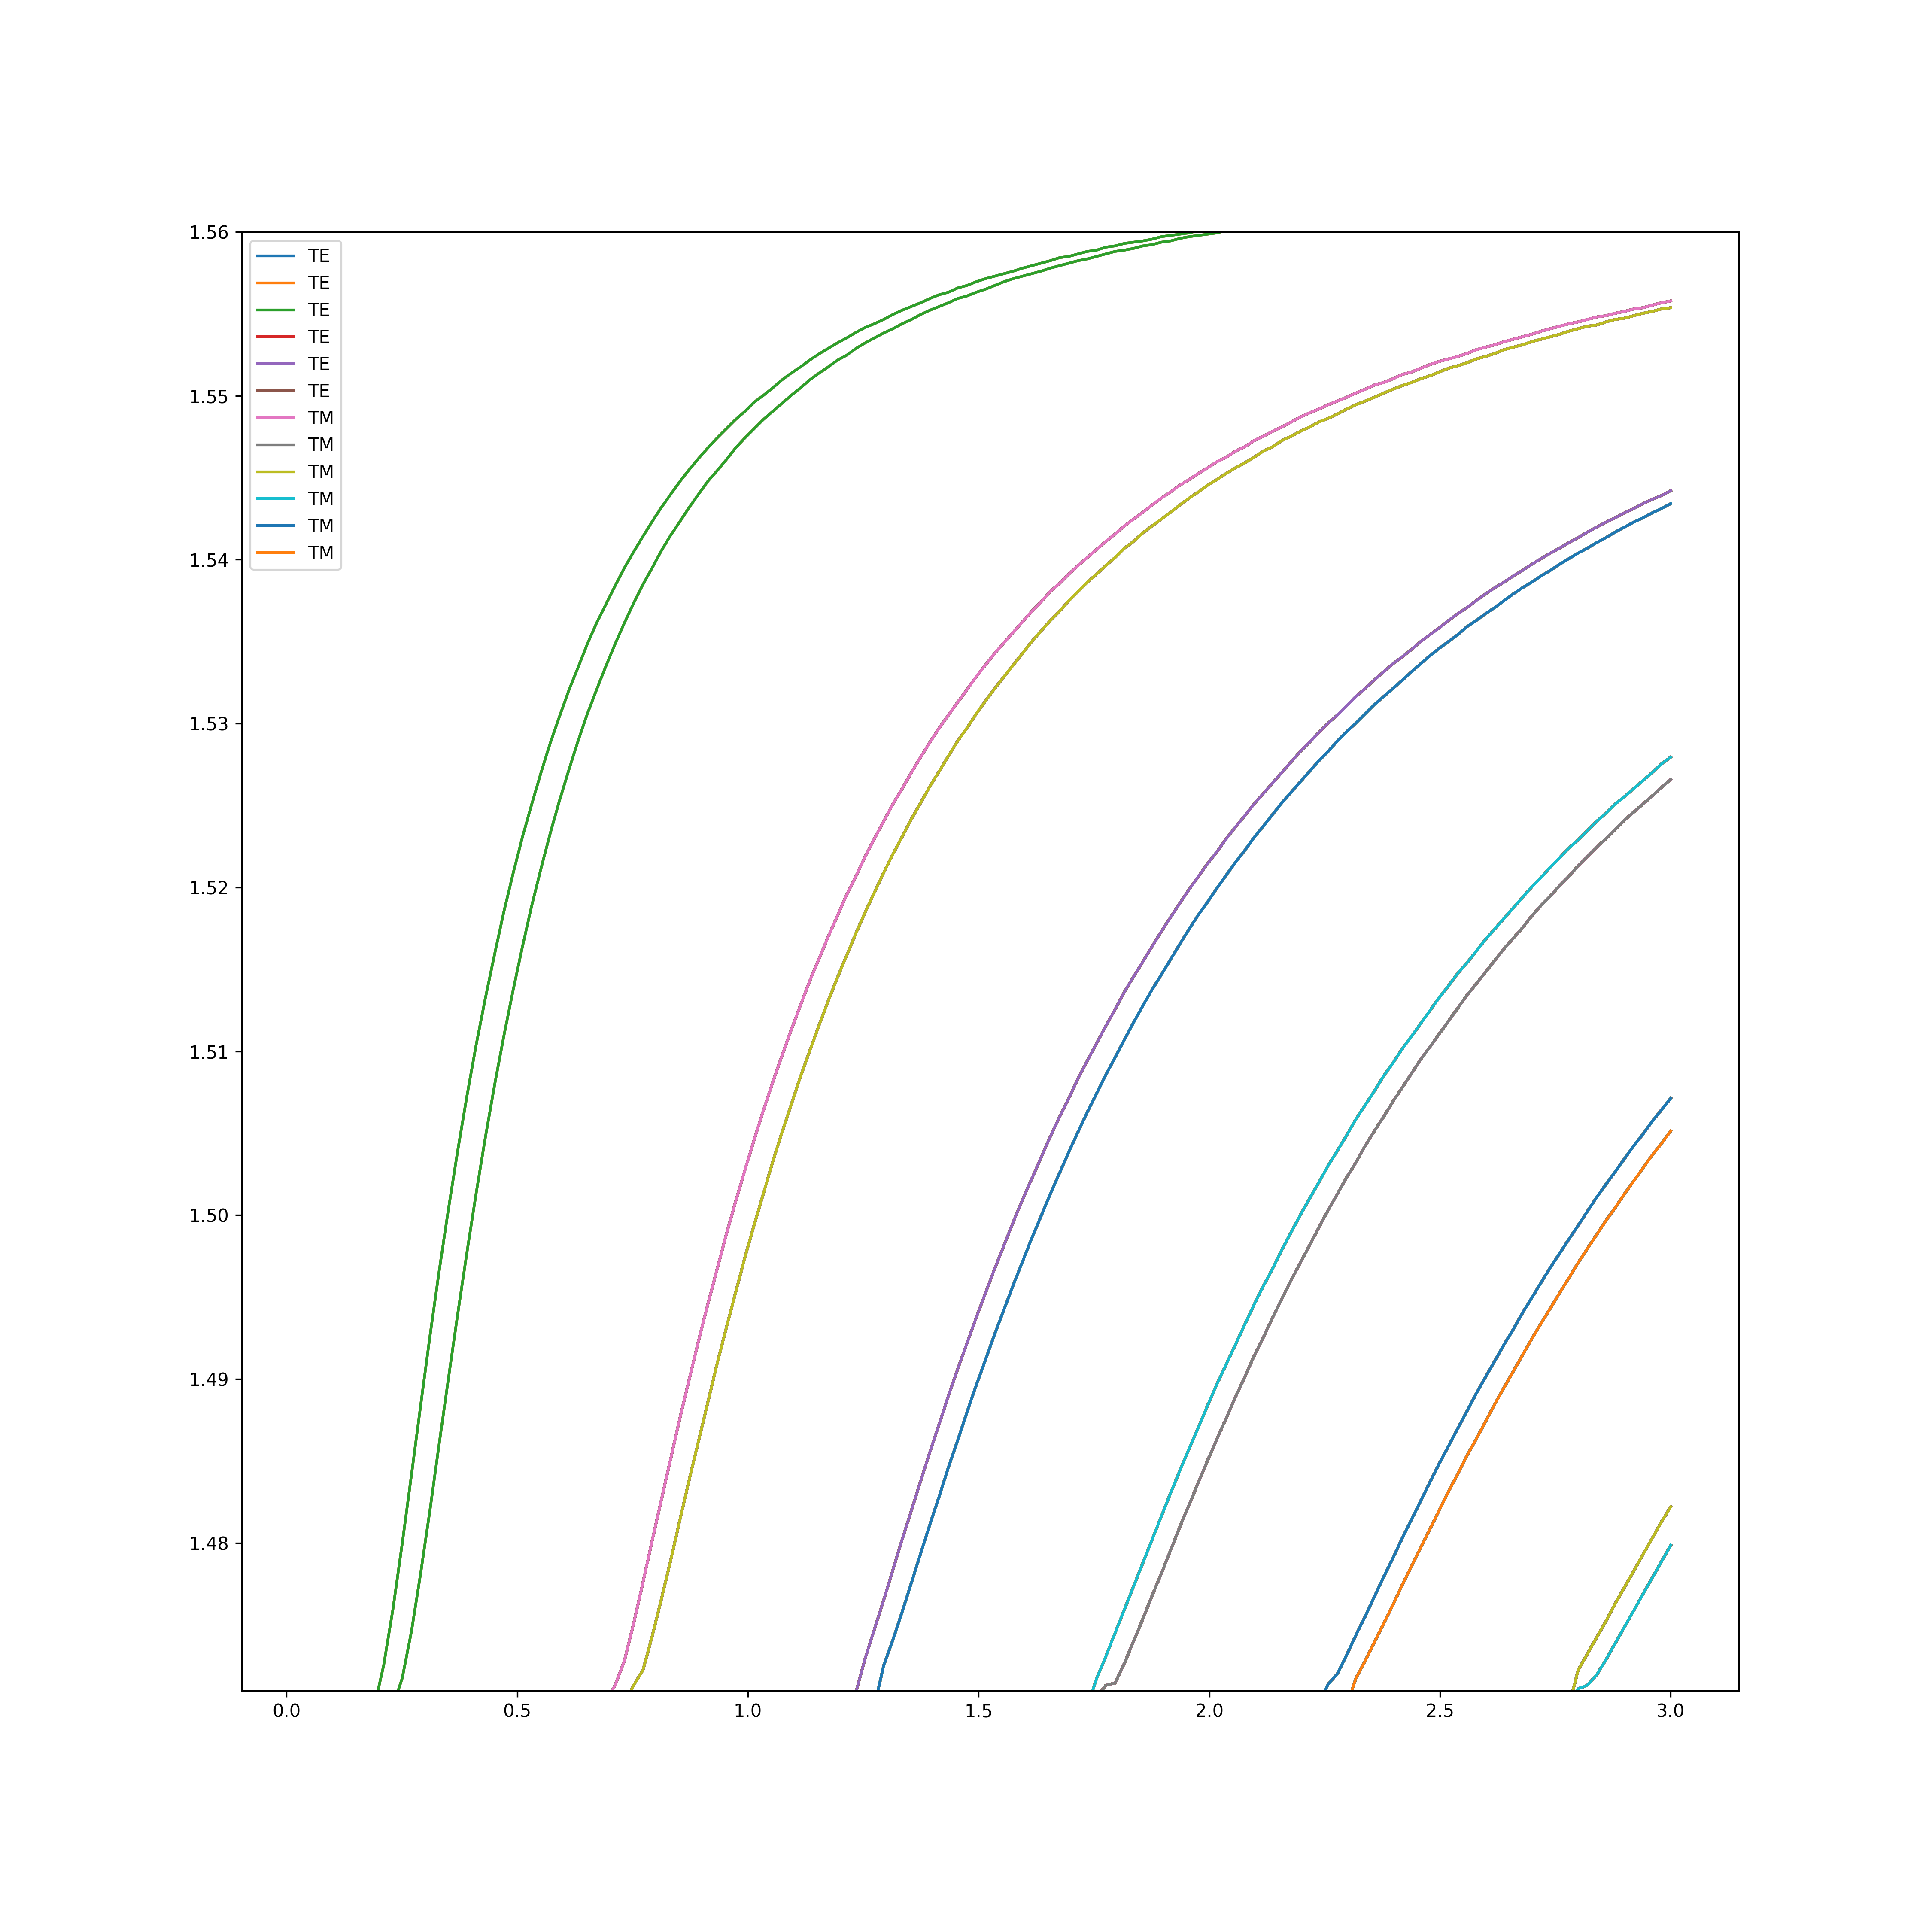
\includegraphics[width=\linewidth]{final.png}
    \caption{Графики $\beta$ от $z$ для мод TE, TM (в каждой паре графиков, одущих близко дргу к другу одна линия принадлежит зависимости в моде TE, другая - зависимости в моде TM)}
    \label{beta_d}
\end{figure}


\newpage

\section{Заключение}

В процессе проектной работы мною были вполнены следующие задачи:
\begin{enumerate}

\item Программирование получения общих решений дифференциальных уравнений 2-го порядка для получения компонент $E_z, H_z$ (раздел 4.1) в средах SymPy и Wolfram Mathematica.
\item Валидация полученных общих решений, сравнение общих решений полученных вручную, с помощью
SymPy и с помощью Wolfram Mathematica.
\item Выведение компонет $E_y, H_y$ из полученных ранее $E_z, H_z$ и их производных по x. Сравнение результатов,
полученных в SymPy и в Wolfram Mathematica.
\item Оформление промежуточных презентаций-отчетов с помощью Google Slides для проектной группы 2.
\item Оптимизация времени работы алгоритма минимизации путем подбора параметров и настройки параллельного выполнения.
\item  Настройка рабочего окружения для сокомандников на сервере.
\item  Написание пунктов 3, 4(4, 4.3, 4.5) отчета. Оформление титульных листов, настройка окружения для
верстки \LaTeX.
\item  Верстка промежуточных результатов(матриц TE,ТМ-мод, матрицы общей СЛАУ) для отчетов.
    
\end{enumerate}
Помимо вышеприведенных задач мною была отработана работа в команде. Изначально мы были разделены на две проектные группы, по три и два человека соответственно. Однако в последствии, из-за сложности
поставленной задачи нами было принято решение обьеденится в одну команду и решать задачу вместе. Это
было в нарушение правил курса, но кажется, что лучше нарушить правила и сдать работу чем не сдать
вообще ничего. В объедененной команде сокрость работы увеличилась заметно, так же был сильный лидер,
распределявший задачи. Это помогло завершить проект лишь с небольшим опозданием от изначального срока сдачи. Мы распределяли задачи относительно своиз умений, в меру возможности работали параллельно
и помогали друг другу освоить материал. Лично мной был обнаружен пробел в собственном умении распределять время на выполнение задач, что несколько раз привело к ошибкам в формировании отчетов. Однако
в результате работы эти пробелы были исправлены.\\[10pt]
Дополнительно, стоит отметить что были получены навыки работы с тяжелыми вычислениями, а именно
оптимизация минимизации $|det(M_{TE})(\beta)|^2$
с целью получения значений коэффициента фазового замедления
$\beta$ при котором СЛАУ $\mathcal{M}_{TE}(\beta, d) \cdot \vec{A}_{TE} = 0$ имело бы нетривиальные решения. Для этого мы разделили диапазон d, которые
фиксировались для поиска $\beta$ на несколько равных промежутков и параллельно запустили минимизации на
этих промежутках на нескольких ядрах процессора. Однако даже распараллеленные вычисления занимали
много времени, поскольку выполнялись на 4х-ядерном процессоре ноутбука. Я предложил перенести вычисления на сервер с двумя 10-ти ядерными процессорами Intel Xeon, который доступен мне для экспериментов.
В результате переноса время работы алгоритма сократилось примерно вчетверо.\\[10pt]
Подводя итог, хочется сказать что проектный тип работы является крайне полезным ввиду того, что
он позволяет отточить как навыки командной работы, так и более узкие навыки в сферах компетенции
отдельных членов команды. Конкретно этот проект был полезен для меня ввиду того, что я развил свои
навыки работы в команде (вместе с одногруппниками) и разобрался с пакетами символьных вычислений и
их оптимизацией




\newpage

\addcontentsline{toc}{section}{Список используемой литературы}
\bibliographystyle{plain}
\bibliography{references.bib}

\newpage

\addcontentsline{toc}{section}{Приложения}
\section*{Приложения}
\subsection*{A - Исходный код}
\begin{lstlisting}[language=Python]

# coding: utf-8

# In[1]:


import math
from scipy.optimize import minimize, newton
import copy
import mpmath

from joblib import Parallel, delayed

import sympy
from sympy import Function, dsolve, Eq,
    Derivative, sin, cos, symbols, pi, I
from sympy.abc import x, y, z

from numba import jit
get_ipython().run_line_magic('matplotlib', 'inline')
sympy.init_session(use_latex=True)

epsilon = symbols("epsilon")
mu = symbols("mu")
lambda_ = symbols("lambda") ## длинна волны света 0.55
k0 = (pi * 2) / lambda_ 

phi = Function("phi")
betta = symbols("beta", real=True)  # Проницаемость среды
betta_y = symbols("beta_y")
betta_z = symbols("beta_z")

betta_y_test = Derivative(phi(y), y) 
betta_z_test = Derivative(phi(z), y)  

E_z = Function('E_z') 
H_z = Function('H_z')

epsilon_s = symbols("epsilon_s") 
mu_s = symbols("mu_s")

Ce_s1 = symbols("C_se1") 
Ce_s2 = symbols("C_se2")  
Ch_s1 = symbols("C_sh1") 
Ch_s2 = symbols("C_sh2") 

eq_s_ez = Derivative(E_z(x), x, x) +
    (k0**2)*(epsilon_s*mu_s - betta**2)*E_z(x)
eq_s_hz = Derivative(H_z(x), x, x) +
    (k0**2)*(epsilon_s*mu_s - betta**2)*H_z(x)

eq_s_ez_sloved = dsolve(eq_s_ez)
eq_s_hz_sloved = dsolve(eq_s_hz)

eq_s_ez_sloved = eq_s_ez_sloved.subs([["C1", Ce_s1], ["C2", Ce_s2]])
eq_s_hz_sloved = eq_s_hz_sloved.subs([["C1", Ch_s1], ["C2", Ch_s2]])


# In[33]:


epsilon_f = symbols("epsilon_f") # Электрическая проницаемость
mu_f = symbols("mu_f")  # Магнитная проницаемостьт

Ce_f1 = symbols("C_fe1") 
Ce_f2 = symbols("C_fe2")  
Ch_f1 = symbols("C_fh1") 
Ch_f2 = symbols("C_fh2")  

eq_f_ez = Derivative(E_z(x), x, x) +
    (k0**2)*(epsilon_f*mu_f - betta**2)*E_z(x)
eq_f_hz = Derivative(H_z(x), x, x) +
    (k0**2)*(epsilon_f*mu_f - betta**2)*H_z(x)

eq_f_ez_sloved = dsolve(eq_f_ez)
eq_f_hz_sloved = dsolve(eq_f_hz)

eq_f_ez_sloved = eq_f_ez_sloved.subs([["C1", Ce_f1], ["C2", Ce_f2]])
eq_f_hz_sloved = eq_f_hz_sloved.subs([["C1", Ch_f1], ["C2", Ch_f2]])

eq_f_hz_sloved = eq_f_hz_sloved.subs({
    betta:betta*I,
    epsilon_f:-epsilon_f,
    pi:pi*I
})

eq_f_ez_sloved = eq_f_ez_sloved.subs({
    betta:betta*I,
    epsilon_f:-epsilon_f,
    pi:pi*I
})

epsilon_c = symbols("epsilon_c") # Электрическая проницаемость
mu_c = symbols("mu_c")  # Магнитная проницаемостьт

Ce_c1 = symbols("C_ce1") 
Ce_c2 = symbols("C_ce2")  
Ch_c1 = symbols("C_ch1") 
Ch_c2 = symbols("C_ch2")  

eq_c_ez = Derivative(E_z(x), x, x) +
    (k0**2)*(epsilon_c*mu_c - betta**2)*E_z(x)
eq_c_hz = Derivative(H_z(x), x, x) +
    (k0**2)*(epsilon_c*mu_c - betta**2)*H_z(x)

eq_c_ez_sloved = dsolve(eq_c_ez)
eq_c_hz_sloved = dsolve(eq_c_hz)

eq_c_ez_sloved = eq_c_ez_sloved.subs([["C1", Ce_c1], ["C2", Ce_c2]])
eq_c_hz_sloved = eq_c_hz_sloved.subs([["C1", Ch_c1], ["C2", Ch_c2]])


left_part = (1 / ((k0**2)*(epsilon_c*mu_c - betta_z**2)))
E_y_c = left_part*(I*k0*mu_c*
    Derivative(H_z(x), x)+(k0**2)*betta_y*betta_z*E_z(x))
H_y_c = left_part*(-(k0**2)*
    betta_y*betta_z*H_z(x)-I*k0*epsilon_c*Derivative(E_z(x), x))
#f
left_part = (1 / ((k0**2)*
    (epsilon_f*mu_f - betta_z**2)))
E_y_f = left_part*(I*k0*mu_f*
    Derivative(H_z(x), x)+(k0**2)*betta_y*betta_z*E_z(x))
H_y_f = left_part*(-(k0**2)*
    betta_y*betta_z*H_z(x)-I*k0*epsilon_f*Derivative(E_z(x), x))
#s
left_part = (1 / ((k0**2)*
    (epsilon_s*mu_s - betta_z**2)))
E_y_s = left_part*(I*k0*mu_s*
    Derivative(H_z(x), x)+(k0**2)*betta_y*betta_z*E_z(x))
H_y_s = left_part*(-(k0**2)*
    betta_y*betta_z*H_z(x)-I*k0*epsilon_s*Derivative(E_z(x), x))

eq_c_hz_diff = diff(eq_c_hz_sloved.rhs,x)
eq_s_hz_diff = diff(eq_s_hz_sloved.rhs,x)
eq_f_hz_diff = diff(eq_f_hz_sloved.rhs,x)
eq_c_ez_diff = diff(eq_c_ez_sloved.rhs,x)
eq_s_ez_diff = diff(eq_s_ez_sloved.rhs,x)
eq_f_ez_diff = diff(eq_f_ez_sloved.rhs,x)

H_y_c = H_y_c.subs({
    H_z(x) : eq_c_hz_sloved.rhs,
    Derivative(E_z(x), x) : eq_c_ez_diff,
})

H_y_f = H_y_f.subs({
    H_z(x) : eq_f_hz_sloved.rhs,
    Derivative(E_z(x), x) : eq_f_ez_diff,
})

H_y_s = H_y_s.subs({
    H_z(x) : eq_s_hz_sloved.rhs,
    Derivative(E_z(x), x) : eq_s_ez_diff,
})

E_y_c = E_y_c.subs({
    E_z(x) : eq_c_ez_sloved.rhs,
    Derivative(H_z(x), x) : eq_c_hz_diff,
})

E_y_f = E_y_f.subs({
    E_z(x) : eq_f_ez_sloved.rhs,
    Derivative(H_z(x), x) : eq_f_hz_diff,
})

E_y_s = E_y_s.subs({
    E_z(x) : eq_s_ez_sloved.rhs,
    Derivative(H_z(x), x) : eq_s_hz_diff,
})

fez_sloved = eq_f_ez_sloved
fhz_sloved = eq_f_ez_sloved

Ez_cf = Equality(eq_c_ez_sloved.rhs - eq_f_ez_sloved.rhs, 0)
Ez_fs = Equality(eq_f_ez_sloved.rhs - eq_s_ez_sloved.rhs, 0)

Hz_cf = Equality(eq_c_hz_sloved.rhs - eq_f_hz_sloved.rhs, 0)
Hz_fs = Equality(eq_f_hz_sloved.rhs - eq_s_hz_sloved.rhs, 0)

Ey_cf = Equality(E_y_c - E_y_f, 0)
Ey_fs = Equality(E_y_f - E_y_s, 0)

Hy_cf = Equality(H_y_c - H_y_f, 0)
Hy_fs = Equality(H_y_f - H_y_s, 0)

Ez_fs = Ez_fs.subs({
    'x': 0, 'beta': betta_z,
    'C_ce2': 0, 'C_ch2': 0,
    'C_se1': 0, 'C_sh1': 0
})
Hz_fs = Hz_fs.subs({
    'x': 0, 'beta': betta_z,
    'C_ce2': 0, 'C_ch2': 0,
    'C_se1': 0, 'C_sh1': 0
})
Ey_fs = Ey_fs.subs({
    'x': 0, 'beta_y': 0,
    'beta': betta_z, 'C_ce2': 0,
    'C_ch2': 0, 'C_se1': 0, 'C_sh1': 0
})
Hy_fs = Hy_fs.subs({
    'x': 0, 'beta_y': 0,
    'beta': betta_z, 'C_ce2': 0,
    'C_ch2': 0, 'C_se1': 0, 'C_sh1': 0
})

d = symbols("d")

Ey_fs_ = Equality(Ey_fs.lhs * 
    (epsilon_s*mu_s - betta_z**2) * 
    (((2*pi)*(epsilon_f*mu_f - betta_z**2))), 0)
.simplify()
Hy_fs_ = Equality(Hy_fs.lhs * 
    (epsilon_s*mu_s - betta_z**2) * 
    (((2*pi)*(epsilon_f*mu_f - betta_z**2))), 0)
.simplify()
Ey_cf_ = Equality(Ey_cf.lhs * 
    (epsilon_c*mu_c - betta_z**2) * 
    (((2*pi)*(2*pi)*(epsilon_f*mu_f - betta_z**2))), 0)
.simplify()
Hy_cf_ = Equality(Hy_cf.lhs * 
    (epsilon_c*mu_c - betta_z**2) * 
    (((2*pi)*(2*pi)*(epsilon_f*mu_f - betta_z**2))), 0)
.simplify()

Ey_fs_new = Equality(Ey_fs_.lhs * 1/(2*pi), 0)
Hy_fs_new = Equality(Hy_fs_.lhs * 1/(2*pi), 0)

Hy_fs_new.expand()

Ez_cf_kek = Ez_cf.subs({
    betta_y : 0,
    Ce_c2 : 0,
    x : d
})
Ez_cf_kek
Hz_cf_kek = Hz_cf.subs({
    betta_y : 0,
    Ch_c2 : 0,
    x : d
})

Hy_cf_kek = Hy_cf_.subs({
    betta_y : 0,
    Ce_c2 : 0,
    betta_z : betta,
    x : d
})
Hy_cf_kek_expand = Hy_cf_kek.expand()
Ey_cf_kek = Ey_cf_.subs({
    betta_y : 0,
    Ch_c2 : 0,
    betta_z : betta,
    x : d
})
Ey_cf_kek_expand = Ey_cf_kek.expand()

L1_kek = sympy.linear_eq_to_matrix(
    [Ez_fs, Hy_fs_new.expand(), Ez_cf_kek, Hy_cf_kek_expand],
    Ce_c1, Ce_f1, Ce_f2, Ce_s2
)[0]
L2_kek = sympy.linear_eq_to_matrix(
    [Hz_fs, Ey_fs_new.expand(), Hz_cf_kek, Ey_cf_kek_expand],
    Ch_c1, Ch_f1, Ch_f2, Ch_s2
)[0]

L1_kek = L1_kek.subs({
    mu_c : 1,
    mu_f : 1,
    mu_s : 1,
    lambda_ : 0.55,
    #h: 2*lambda_,
    betta_z: betta,
    epsilon_c : 1,
    epsilon_f : 1.565 ** 2,
    epsilon_s : 1.47 ** 2
})

L2_kek = L2_kek.subs({
    mu_c : 1,
    mu_f : 1,
    mu_s : 1,
    lambda_ : 0.55,
    #h: 2*lambda_,
    betta_z: betta,
    epsilon_c : 1,
    epsilon_f : 1.565 ** 2,
    epsilon_s : 1.47 ** 2
})

omg = L1_kek.det()
omg2 = L2_kek.det()

class DBettaAdapter:
    def __init__(self, left, right, determinant, d_):
        self.init_right_bound = right
        self.init_left_bound = left
        self.raw_deterninant = determinant
        self.set_d(d_)
        self.factor = 1
        self.epsilon = 1e-6
        self.min = []
    
    def set_d(self, d_):
        self.determinant = self.raw_deterninant.subs({"d":d_})
        self.d = d_

    def set_bounds(self, left, right):
        self.right_bound = right
        self.left_bound = left
    
    def func(self, b):
        b = b[0]
        eval_ = self.determinant.evalf(subs={betta:b})
        if b < self.left_bound or b > self.right_bound:
            return 1000
        else:
            ans = mpmath.power(Abs(eval_), 2)
        return ans * self.factor

    def opt(self):
        mid = (self.right_bound - self.left_bound)/2 + self.left_bound
        res = minimize(self.func, [mid], method ="BFGS")#
        return res
    
    def draw_plot(self, num_points=100):
        #for i in arr:
        #    res_.append(self.func([i]))
        arr, step, res_ = self.eval_array(num_points)
        
        plt.plot(arr, np.array(res_, dtype=np.float64))
        plt.xlabel("betta")
        plt.ylabel('determinant')
        plt.show()
    
    def eval_array(self, num_points=100):
        res_ = []
        arr = np.linspace(self.left_bound, self.right_bound, num_points)
        step = arr[1] - arr[0]
        for i in arr:
            res_.append(self.func([i]))
        return arr, step, np.array(res_)
    
    @staticmethod
    def find_local_min(arr):
        diff = np.diff(arr)
        res = []
        for i in range(len(diff)-1):
            #print(diff[i], diff[i+1], i)
            if diff[i]<0 and diff[i+1]>0:
                res.append(i)
        return res
    
    def get_mins(self, num_points=100):
        arr, step, res_ = self.eval_array(num_points)
        init_mins = self.find_local_min(res_)
        
        local_mins = []
        start = copy.deepcopy(self.left_bound)
        for min_ in init_mins:
            left_bound = start + min_ * step
            right_bound = start + (min_ + 3) * step
            #print(left_bound, right_bound)
            self.set_bounds(left_bound, right_bound)
            opt_result = self.opt()
            local_mins.append([opt_result.x, opt_result.fun])
        return local_mins
    
    def find_min_d_range(self, d_array, num_points=100):
        result = []
        for d in d_array:
            self.set_d(d)
            self.set_bounds(self.init_left_bound, self.init_right_bound)
            mins_ = [i[0] for i in self.get_mins(num_points)]
            result.append([d, mins_])
        return result
    
    def find_min_d_range_parallel(self, d_array, num_points=100):
        result = Parallel(n_jobs=16)(delayed(self.parallel_adapter)
            (i, num_points) for i in d_array)
        return result
    
    def parallel_adapter(self, d, num_points=100):
            self.set_d(d)
            self.set_bounds(self.init_left_bound, self.init_right_bound)
            mins_ = self.get_mins(num_points)
            #mins_ = [i[0] for i in self.get_mins(num_points)]
            return d, mins_

k = DBettaAdapter(1.4695, 1.56505, omg, 1)

d_arr = np.linspace(0.1, 2, 10)

get_ipython().run_cell_magic(
    'time', '',
    'k = DBettaAdapter(1.4695, 1.56505, omg, 1)\nd_arr = 
    np.linspace(0.01, 3, 150)\nres 
    = k.find_min_d_range_parallel(d_arr, 150)'
)

get_ipython().run_cell_magic(
    'time', '',
    'k2 = DBettaAdapter(1.4695, 1.56505, omg2, 1)\nd_arr =
    np.linspace(0.01, 3, 150)\nres2 
    = k2.find_min_d_range_parallel(d_arr, 150)'
)

def pad(arr, d_s):
    target = len(d_s) - len(arr)
    return d_s[target:], np.pad(np.array(arr), [target, 0], "edge")[target:]

matplotlib.rcParams['figure.dpi'] = 300

def split_increasing_array(arr):
    res = []
    new_res = []
    for i in range(len(arr)-1):
        if arr[i]>arr[i+1]:
            new_res.append(arr[i])
            res.append(new_res)
            new_res = []
        else:
            new_res.append(arr[i])
    new_res.append(arr[i+1])
    res.append(new_res)
    return res

_ = plt.figure(figsize=(15.0, 15.0))

plt.ylim(1.471, 1.56)
legend = []
bettas = [[] for _ in range(len(res[-1][-1]))]
d_s = [i[0] for i in res]
for d, betta_s in res:
    for betta_i in range(len(betta_s)):
        bettas[betta_i].append(betta_s[betta_i][0])

target = list(map(split_increasing_array, bettas))
for i in range(6):
    m = []
    for j in target:
        try:
            m.extend(j[i])
        except: pass
    d_s = [i[0] for i in res]
    d_s, pad_ = pad(m, d_s)
    plt.plot(d_s, pad_)
    legend.append('TE')
    
bettas = [[] for _ in range(len(res2[-1][-1]))]
d_s = [i[0] for i in res2]
for d, betta_s in res2:
    for betta_i in range(len(betta_s)):
        bettas[betta_i].append(betta_s[betta_i][0])

target = list(map(split_increasing_array, bettas))
for i in range(6):
    m = []
    for j in target:
        try:
            m.extend(j[i])
        except: pass
    d_s = [i[0] for i in res2]
    d_s, pad_ = pad(m, d_s)
    plt.plot(d_s, pad_)
    legend.append('TM')

plt.legend(legend)

plt.savefig("./final.png")

\end{lstlisting}

\end{document}
